\chapter{Addytywna synteza dźwięku}\label{chapter_additive}
Synteza addytywna pozwala na utworzenie barwy dźwięku poprzez zbudowanie pełnego widma częstotliwościowego za pomocą odpowiednich składowych. Słowo 'addytywna' odnosi się do sumowania wielu przebiegów w jeden złożony sygnał dźwiękowy. Historycznie jest ona drugą najstarszą metodą syntezy, zaraz po subtraktywnej, opisanej w rozdziale \ref{chapter_subtractive}.
Zazwyczaj synteza addytywna polega na dodawaniu wielu fal sinusoidalnych o różnych częstotliwościach oraz amplitudach. Metoda ta pozwala jednak na dużą dowolność. Dodawanymi składowywmi sygnału nie muszą być jedynie fale sinusoidalne.
Synteza addytywna uznawana jest za odwrotność syntezy subtraktywnej. Znajduje zastosowanie w syntezie dźwięku oraz mowy.

W niniejszym rozdziale przedstawiono zasadę działania syntezy addytywnej. Zaprezentowano wzory matematyczne, za pomocą których można uzyskać zsyntezowane brzmienie. Przedstawiono również kilka metod implementacji tego rodzaju syntezy. Na końcu rozdziału zaprezentowano autorski interfejs użytkownika oraz wyniki zaimplementowania syntezy addytywnej na procesorze DSP.

\section{Zasada działania syntezy addytywnej}
Synteza addytywna jest zbliżona pod niektórymi względami do analizy częstotliwościowej Fouriera. Z tego powodu jest ona zaliczana do widmowych metod syntezy. Jej postać matematyczną można jednak przedstawić w dziedzinie czasu. Zależnie od doboru składowych dźwięku, przedstawienie syntezy addytywnej może różnie wyglądać.
% Okresowosc sygnalu y(t)
%https://ccrma.stanford.edu/~jos/sasp/Additive_Synthesis_Early_Sinusoidal.html

\subsection{Postać harmoniczna} \label{pos_harm}
Dźwięk powstały w wyniku użycia syntezy addytywnej w formie harmonicznej można zapisać w postaci:
%https://en.wikipedia.org/wiki/Additive_synthesis#:~:text=Additive%20synthesis%20is%20a%20sound,or%20inharmonic%20partials%20or%20overtones.
\begin{equation} \label{equ:addit_time_harm}
y(t) = \sum_{k=1}^{K} a_{k}sin(2\pi kf_{0}t + \phi_{k})  \\  
\end{equation}
\begin{tabular}{ l l l l}
	gdzie: & $y(t)$ &  - & wyjście addytywnej syntezy dźwięku, \\
	&	$k$ & - &  numer składowej harmonicznej sygnału, \\
	&	$K$ & - &  całkowita liczba składowych harmonicznych dźwięku,\\
	&	$f_{0}$ & - &  częstotliwość pierwszej składowej harmonicznej,\\
	&	$a_{k}$ & - &  amplituda składowej harmonicznej k, \\
	&	$\phi_{k}$ & - &  faza składowej harmonicznej k. \\
\end{tabular}

Każda składowa dźwięku uzyskanego z tej postaci syntezy addytywnej jest wielokrotnością częstototliwości podstawowej $f_{0}$. Wykorzystanie takiej postaci pozwala na utworzenie dźwięku na przykład organów. Jest to najbardziej podstawowy rodzaj syntezy addytywnej.

%https://en.wikibooks.org/wiki/Sound_Synthesis_Theory/Additive_Synthesis <<---- SCHEMAT 

%https://en.wikipedia.org/wiki/Square_wave
\begin{equation} \label{equ:addit_sqr}
y_{Square}(t) = \sum_{k=1}^{K} \frac{1}{2k-1} sin(2\pi (2k-1)f_{0}t) \\
\end{equation}

%https://en.wikipedia.org/wiki/Triangle_wave
\begin{equation} \label{equ:addit_trng}
y_{Triangle}(t) = \sum_{k=1}^{K} \frac{(-1)^k}{(2k-1)^2} sin(2\pi (2k-1)f_{0}t)  \\
\end{equation}

%https://en.wikipedia.org/wiki/Sawtooth_wave
\begin{equation} \label{equ:addit_sawth}
y_{Sawtooth}(t) = \sum_{k=1}^{K} \frac{(-1)^k}{k} sin(2\pi kf_{0}t) \\
\end{equation}
% O tym że na tym polegały organy Hammonda

Postać harmoniczna syntezy addytywnej pozwala również na uzyskanie podstawowych przebiegów używanych w syntezie subtraktywnej. Każdy z nich można wygenerować za pomocą sumowania odpowiednich składowych harmonicznych z odpowiednimi amplitudami. Przykłady takich przebiegów przedstawiono we wzorach \ref{equ:addit_sqr}, \ref{equ:addit_trng} oraz \ref{equ:addit_sawth}.

\begin{figure}[H]
	\centering
	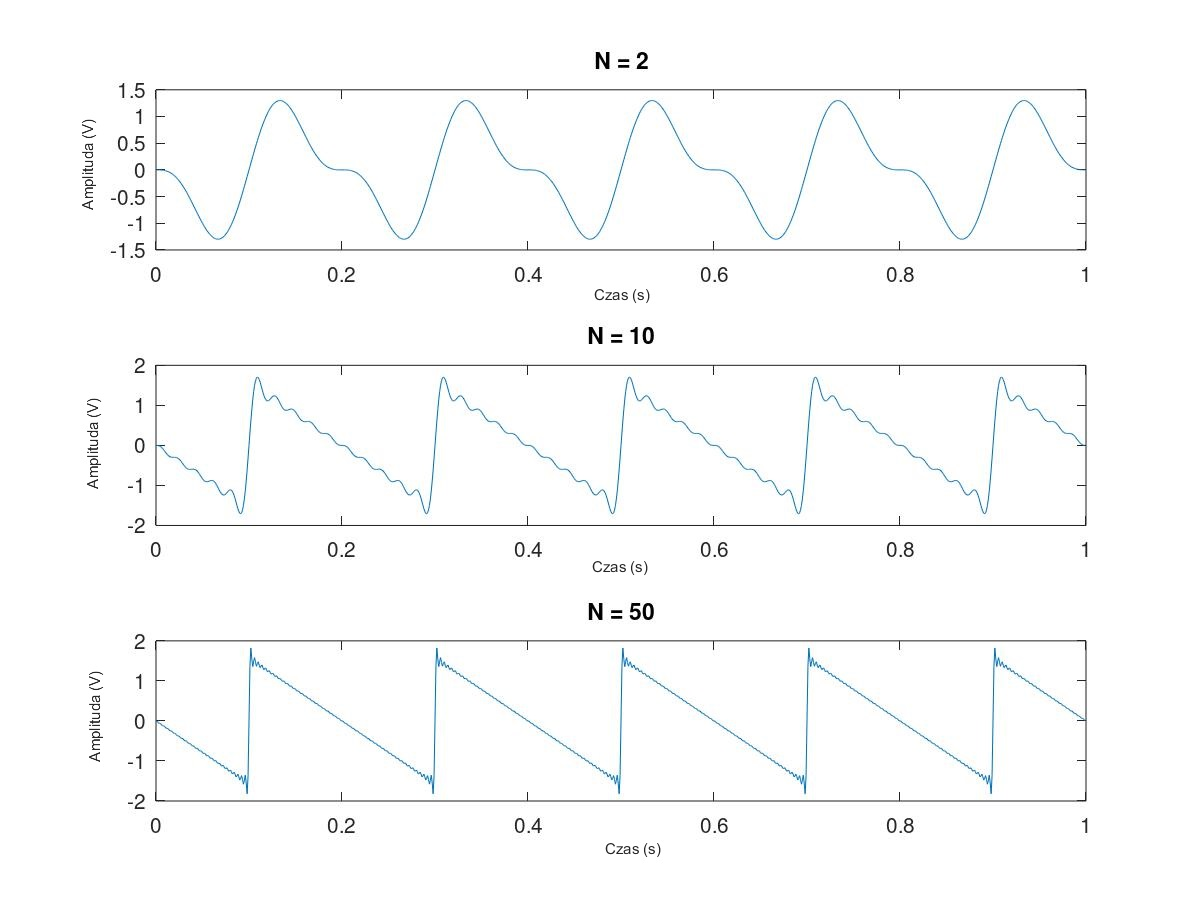
\includegraphics[width=12cm]{grafiki/add_sawtooth}
	\captionsetup{justification=centering}
	\caption{Generacja przebiegu piłokształtnego za pomocą syntezy addytywnej.}
	\label{rys:add_sawtooth}
\end{figure}

Na rysunku \ref{rys:add_sawtooth} przedstawiono generowanie przebiegu piłokształtnego, jako przykład addytywnej syntezy dźwięku w postaci harmonicznej. Na pierwszym z wykresów przedstawiono przebieg uzyskany z dwóch składowych harmonicznych, a na kolejnym z 10. Na ostatnim wykresie widać przebieg składający się z 50 SH, który jest dobrą aproksymacją idealnego przebiegu piłokształtnego. Amplitudy kolejnych składowych tego sygnału obliczone zostały na podstawie wzoru \ref{equ:addit_sawth}

\subsection{Postać nieharmoniczna} \label{pos_nieharm}
Dobieranie składowych dźwięku w syntezie addytywnej nie musi zależeć od konkretnej częstotliwości. Niektóre instrumenty wydają dźwięk składający się ze składowych harmonicznych i nieharmonicznych (czyli takich, które nie są całkowitą wielokrotnością pewnej częstotliwości $f_{0}$). Zsyntezowany dźwięk w takiej postaci można opisać wzorem:
\begin{equation} \label{equ:addit_time_nieharm}
y(t) = \sum_{k=1}^{K} a_{k}sin(2\pi f_{k}t + \phi_{k})  \\  
\end{equation}
\begin{tabular}{ l l l l}
	gdzie: 	&	$f_{k}$ & - &  częstotliwość składowej sygnału k,\\
\end{tabular}

Dźwięk opisany powyższym wzorem jest generowany przez instrumenty takie jak dzwony lub perkusjonalia.

\subsection{Składowe zmienne w czasie}
%https://books.google.pl/books/about/The_Computer_Music_Tutorial.html?id=nZ-TetwzVcIC&printsec=frontcover&source=kp_read_button&redir_esc=y#v=onepage&q&f=false
Wzory matematyczne \ref{equ:addit_time_harm} i \ref{equ:addit_time_nieharm} pozwalają na uzyskanie jedynie stanu ustalonego zsyntezowanego brzmienia. Powtarzany jest jeden okres sygnału, co daje wrażenie słuchaczowi, iż barwa dźwięku jest bardzo prosta.

Składowe dźwięku mogą jednak zmieniać się w czasie. Zmiany te mogą dotyczyć zarówno ich amplitudy, jak i częstotliwości. Synteza addytywna ze zmi
Taką postać syntezy addytywnej zapisuje się:
\begin{equation} \label{equ:addit_time_zmienne}
y(t) = \sum_{k=1}^{K} a_{k}(t)sin(2\pi f_{k}(t)t + \phi_{k})  \\  
\end{equation}
\begin{tabular}{ l l l l}
	gdzie: & $a_{k}(t)$ &  - & zmienna w czasie amplituda składowej k, \\
	&	$f_{k}(t)$ & - &  zmienna w czasie częstotliwość składowej k, \\
\end{tabular}

\subsection{Szum w syntezie addytywnej}
%https://ccrma.stanford.edu/~jos/sasp/S_N_Synthesis.html
Tworzenie sygnału zsyntezowanego metodą addytywną za pomocą wzorów przedstawionych powyżej jest deterministyczne. Do takiego sygnału można dodać jednak część stochastyczną. Uzyskuje się to z wykorzystaniem zmiennego w czasie filtra FIR oraz białego szumu.

\begin{equation} \label{equ:addit_szum}
B(\omega) = F(\omega)*e^{j\phi(\omega_{k})} \\  
\end{equation}
\begin{tabular}{ l l l l}
	gdzie: & $\phi(\omega_{k})$ &  - & faza losowa o rozkładzie równomiernym, \\
	& $F(\omega)$ &  - & obwiednia widmowa filtra FIR, \\
	&	$B(\omega)$ & - & zmienna w czasie częstotliwość składowej k, \\
\end{tabular}

Synteza części stochastycznej polega na przepuszczeniu białego szumu (bazującego na losowej fazie) przez filtr FIR. Takie działanie zostało zaprezentowane we wzorze \ref{equ:addit_szum}.
Dodanie szumu do sygnału deterministycznego w syntezie addytywnej pozwala na uzyskanie dźwięków na przykład instrumentów dętych.

\section{Metody implementacji syntezy addytywnej}

Istnieją różne metody implementacji addytywnej syntezy dźwięku. Ten sam dźwięk może być uzyskany różnymi sposobami. Popularne metody realizacji syntezy addytywnej to:
\begin{itemize}
	\item bank oscylatorów,
	\item synteza wavetable,
	\item synteza IFFT.
	% https://ieeexplore.ieee.org/document/4412805 86zł
\end{itemize}

\subsection{Ograniczenia syntezy addytywnej} \label{addit_ograniczenia}
%https://en.wikipedia.org/wiki/Additive_synthesis#History
Synteza addytywna w instrumentach klawiszowych jest używana między innymi do generacji dźwięku organów, których barwa upraszczana jest zazwyczaj do kilku SH. W przypadku próby uzyskania dźwięku o większej ilości składowych harmonicznych, złożoność obliczeniowa metody wzrasta.
%https://ccrma.stanford.edu/~jos/pasp/Additive_Synthesis.html
Przykładowo, dla uzyskania pojedynczego dźwięku pianina w jakości CD-Audio,
%https://en.wikipedia.org/wiki/Compact_Disc_Digital_Audio
wymagane byłoby obliczenie około 400 fal sinusoidalnych na każdą próbkę zsyntezowanego dźwięku. Oznacza to, iż dla polifonicznej klawiatury takiego pianina, byłyby to tysiące składowych. Obecne ograniczenia sprzętowe nie pozwalają na szybki rozwój addytywnej metody syntezy dźwięku, gdyż jest ona bardzo złożona obliczeniowo.

\subsection{Bank oscylatorów}
%analogowe hammondy i zwykłe, ale ze są wolne
Synteza przez bank oscylatorów jest najstarszą metodą implementacji addytywnej syntezy dźwięku. Opiera się ona bezpośrednio na równaniu \ref{equ:addit_time_harm}.
Ta metoda implementacji realizowana była nawet na instrumentach analogowych. Instrumenty takie jak organy Hammonda posiadały kilka dyskowych wirników, które były nacięte w kilku miejscach na ich powierzchni. Obracające wirniki generowały prąd elektryczny o charakterystyce zawierającej pewne składowe harmoniczne tonu podstawowego.

Implementacja na procesorach DSP, odpowiadająca dyskowym wirnikom, opiera się na realizowaniu wielu funkcji sin() o różnych częstotliwościach i amplitudach. Każda taka funkcja generuje jedną składową harmoniczną syntezowanego dźwięku. Wszystkie razem traktowane są jako bank oscylatorów. Problem realizacji skomplikowanego brzmienia takim sposobem został przedstawiony w punkcie \ref{addit_ograniczenia}.

\begin{figure}[H]
	\centering
	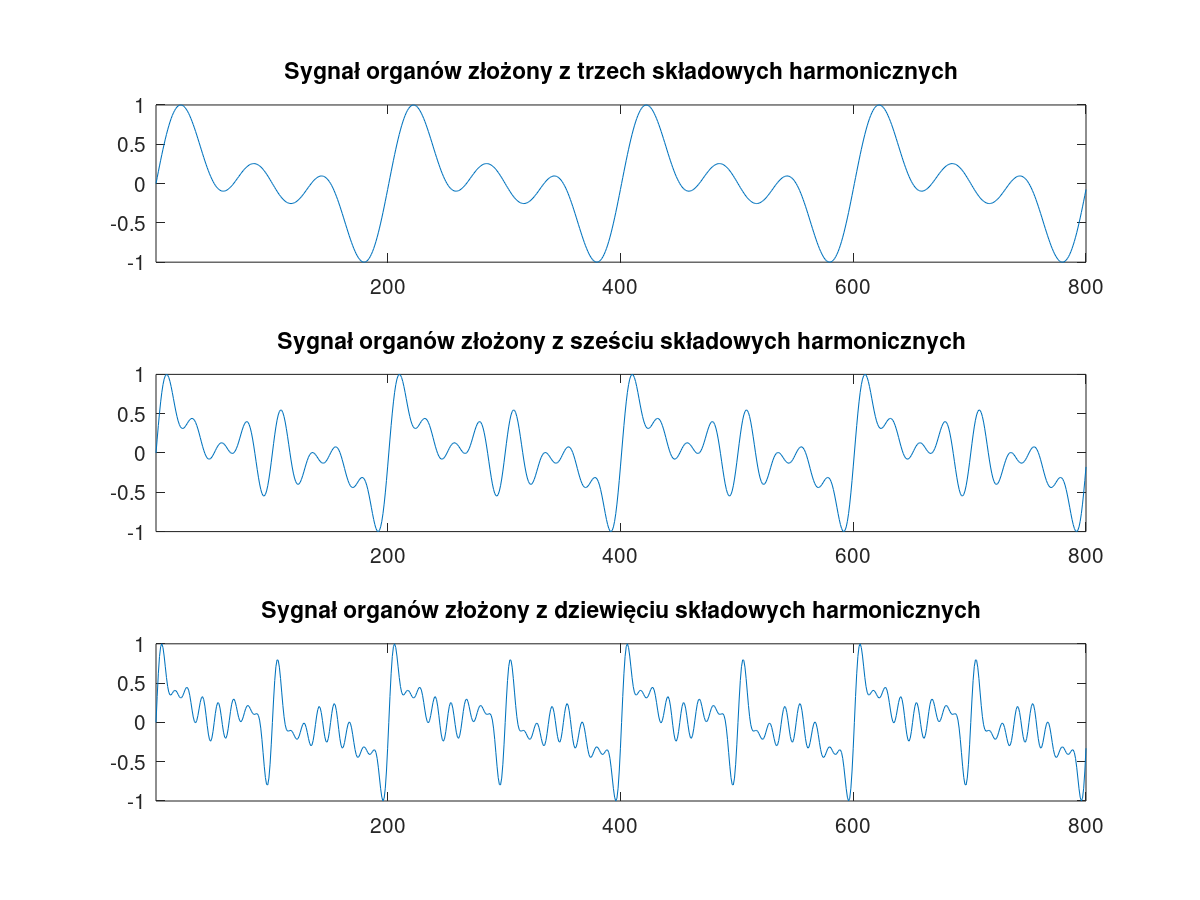
\includegraphics[width=15cm]{grafiki/add_hammond_matlab}
	\captionsetup{justification=centering}
	\caption{Barwa dźwięku organów Hammonda dla różnych ilości składowych harmonicznych.}
	\label{rys:add_hammond_matlab}
\end{figure}

Na rysunku \ref{rys:add_hammond_matlab} przedstawiono wygenerowaną barwę organów Hammonda dla trzech różnych ustawień amplitud składowych harmonicznych.


\subsection{Synteza wavetable} \label{add_wavetable}
%opisac tą która została zaimplementowana
Synteza wavetable (nazywana również syntezą tablicową lub lookup-table) polega na zapisaniu jednego okresu fali dźwiękowej do tablicy zdefiniowanej w programie komputerowym. W każdej kolejnej chwili czasu działania programu, odczytywany jest odpowiedni element tablicy. Okres fali zapisanej w tablicy powinien zawierać nadmierną liczbę próbek (ang. over-sampled), aby móc odczytać go dla niskich częstotliwościach. Niewystarczające spróbkowanie może doprowadzić do znacznych skoków wartości generowanej fali za pomocą metody wavetable.

W syntezie addytywnej użycie takiej metody implementacji może znacznie przyspieszyć generowanie kolejnych próbek składowych sygnału. Do tablicy zapisuje się jeden przebieg sinusoidalny. Odczyt jednego indeksu zabiera mniej czasu pracy procesora niż wygenerowanie próbki z funkcji sin(). Działanie takiej metody jest podobne do banku oscylatorów, ze względu na to, iż również realizowana jest w dziedzinie czasu. Znaczna różnica jest taka, że tablicę w syntezie wavetable można traktować jako jeden oscylator, z którego należy jedynie odczytać wartości tj. znaleźć odpowiedni indeks tablicy. Nie trzeba w każdej chwili czasu obliczać na nowo próbki dla każdej składowej dźwięku.
%https://en.wikipedia.org/wiki/Lookup_table

\subsection{Synteza IFFT}
%Rysunki z matlaba
W 1990 roku P. Depalle oraz X. Rodet przedstawili przełomową metodę implementacji syntezy addytywnej. W ich podejściu obliczanie składowych nie opiera się na zestawie oscylatorów, lecz na algorytmie IFFT (ang. Inverse Fast Fourier Transform) stosowanym dla krótkiego okna widma (STS, ang. short term spectrum). Wyniki ich pracy dowiodły, iż zmniejszyli koszt obliczeń syntezy addytywnej piętnastokrotnie, w stosunku do oscylatorów sinusoidalnych (w ich indywidualnym przypadku, gdzie obliczali 9 istotnych punktów widma w 256 próbkowym STS).

Konstrukcja pojedynczej ramki STS została przedstawiona poniżej. Niech $f_{j}$, $a_{j}$ oraz $\phi_{j}$ będą średnimi wartościami częstotliwości, amplitudy i fazy ramki czasowej pożądanego sygnału $w[n]$. $W$ niech będzie Transformatą Fouriera okna sygnału $w[n]$. Wtedy dodanie pojedynczej składowej do STS może być zapisana jako:

\begin{equation} \label{equ:addit_IFFT}
S[k] = a_{j}e^{i\phi_{j}}W[f_{j} - k] \\  
\end{equation}
\begin{tabular}{ l l l l}
	gdzie: & $S[k]$ &  - & STS syntezowanego sygnału, \\
	& $W[f_{j} - k]$ &  - & przesunięte widmo sygnału $w[n]$, \\
	& $a_{j}e^{i\phi_{j}}$ & - & zespolona amplituda. \\
\end{tabular}

Wzór \ref{equ:addit_IFFT} oznacza, iż okno widmowe $W[f_{j} - k]$ zostanie wycentrowane na częstotliwości $f_{j}$ oraz przemnożonę przez amplitudę $a_{j}e^{i\phi_{j}}$. Po takim działaniu w dziedzinie częstotliwości, okno STS poddane jest algorytmowi IFFT, którego rezultatem jest okno czasowe $s[n]$. Kolejne okna czasowe zakładkowane są metodą overlap-add.

Dodanie szumu do sygnału w przypadku syntezy addytywnej za pomocą metody IFFT jest również bardziej efektywne obliczeniowo. Szum biały może zostać dodany już na etapie tworzenia STS, a następnie poddany algorytmowi IFFT. Ostatecznie uzyskiwane jest okno sygnału zawierającego część deterministyczną, jak i stochastyczną.

\section{Interfejs użytkownika}
W autorskim projekcie, w ramach realizacji instrumentu klawiszowego z syntezą addytywną, zaimplementowano program generujący dźwięk organów Hammonda. 
%https://www.soundonsound.com/techniques/synthesizing-tonewheel-organs-part-1
Laurens Hammond, twórca tychże organów, zaprojektował je tak, aby użytkownik miał możliwość doboru amplitudy dziewięciu składowych harmonicznych generowanego dźwięku. Każda z nich była regulowana gałką na 8 poziomach. Gałki oznaczały kolejno wartości amplitudy pierwszej, drugiej, trzeciej, czwartej, szóstej, ósmej, dziesiątej, dwunastej oraz szesnastej składowej harmonicznej dźwięku. Przykładowe różnice w generowanej barwie organów przedstawione zostały na rysunku \ref{rys:add_hammond_matlab}.

\begin{figure}[H]
	\centering
	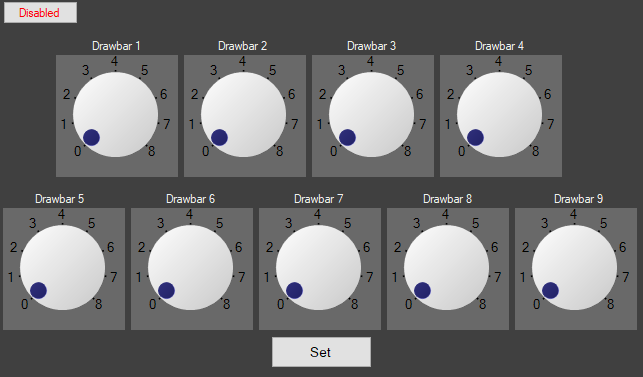
\includegraphics[width=15cm]{grafiki/add_interface}
	\captionsetup{justification=centering}
	\caption{Interfejs użytkownika dla syntezy addytywnej.}
	\label{rys:add_interface}
\end{figure}

Interfejs użytkownika opiera się na oryginalnym instrumencie Laurensa Hammonda. Umożliwia on użytkownikowi regulację dziewięciu SH za pomocą gałek przedstawionych na rysunku \ref{rys:add_interface}. Można zauważyć, iż gałki posiadają również 8 poziomów wartości, które odpowiadają wartościom amplitud składowych harmonicznych. Po ustawieniu pożądanej barwy, użytkownik musi kliknąć w panelu przycisk "Set", aby parametry syntezy addytywnej zostały wysłane do procesora DSP.

Gałki w panelu zostały zrealizowane za pomocą obiektów klasy KnobControl. Naciśnięcie przycisku "Set" wywołuje funkcję, która odczytuje wartość elementu panelu syntezy addytywnej w formie tablicy bajtów. Następnie wysyła odpowiedni identyfikator gałki, a po nim jej wartość.

\section{Implementacja na procesorze DSP}
W autorskim programie komputerowym na procesor DSP wykorzystano metodę implementacji z użyciem tablicy wavetable, która została omówiona w \ref{add_wavetable}. 